\section{Supplementary Empirical Results for Non-Adaptive and Adaptive Experiments}\label{sec:supplementary-empirical}

\subsection{Data Description}\label{subsec:description-data-sets}

We first provide more details about the flu data. We use ICD-9 diagnosis codes to select the inpatient and outpatient records whose primary diagnosis of the patient is influenza.\footnote{These databases only have claim records with ICD-9 diagnosis codes.} The ICD-9 diagnosis codes for influenza are 488, 487.0, 487.1, 487.8, 488.0, 488.1, 488.01, 488.02, 488.09, 488.11, 488.12, 488.19, 488.81, 488.82, and 488.89.
Since these are claims data, unlike electronic medical records that may be restricted to only a few healthcare providers, we can see all clinical visits of every patient for the duration of their enrollment. Empowered by this unbiased coverage of patient visits in our data, we observe that patients are not typically admitted to hospitals for influenza, as there are 21,277 inpatient admissions versus 9,678,572 outpatient visits with primary diagnosis influenza. We denote all of these as influenza visits. 

Next, we provide further details about the three data sets, home medical visits, grocery store transactions, and Lending Club data, initially introduced in Section \ref{subsec:data-description}.
\begin{itemize}
    \item Home medical visits data set has 40,079 records of home medical visits from Jan 2016 to Dec 2018 in the metropolitan area of Barcelona Spain.\footnote{This data set is publicly available on Kaggle and can be downloaded at \url{https://www.kaggle.com/ckroxigor/home-medical-visits-eda/}.} This data set has been used to study how environmental factors adversely affect vulnerable people to environmental agents (climate, pollution, etc). We aggregate this data at the city level, as many environmental policies are carried out at an aggregate level. Given the high noise in the number of visits, we consider the 16-week moving average of medical visits. Then we obtain a panel of $61$ cities across $144$ weeks.


\item Grocery store transactions data set contains 17,880,248 transactions from a large grocery store between May 2005 and May 2007.\footnote{This data set is available to researchers at Stanford and Berkeley by application. Papers that use this data set are available at \url{https://are.berkeley.edu/SGDC/publications.html}.} We aggregate the transactions by household and week. Our analysis focuses on ``frequent'' households, defined as those who had expenditures in at least half of the weeks in the data set. These households tend to pay more attention to changes in the loyalty program. We then obtain a panel of $7,130$ frequent households over $97$ weeks. 


\item Lending Club loan data contains 2,260,668 loans issued from June 2007 to December 2018 on Lending Club.\footnote{This data set can be downloaded at \url{https://www.kaggle.com/wordsforthewise/lending-club}}   This data set contains information, such as the current loan status (Current, Late, Fully Paid, etc.), latest payment information, first three digits of zip codes and issued month. We aggregate the number of loans issued by month and by the first three digits of zip codes. We get a panel of $956$ units over $139$ months.

\end{itemize}



\subsection{Supplementary Results for Non-Adaptive Experiments}


\subsubsection{Robustness to Additional Data Sets}\label{subsubsec:robustness-additional-data-set}
Figure \ref{fig:additional-varying-N} shows that the three findings in Section \ref{subsec:fixed-sample-empirical-results} continue to hold on the other three data sets, as $N$ is varied. Figure \ref{fig:additional-varying-T} shows the three findings in Section \ref{subsec:fixed-sample-empirical-results} continue to hold on all four data sets, as $T$ is varied. 



\begin{figure}[H]
	\centering
	\begin{subfigure}{1\textwidth}
		\centering
		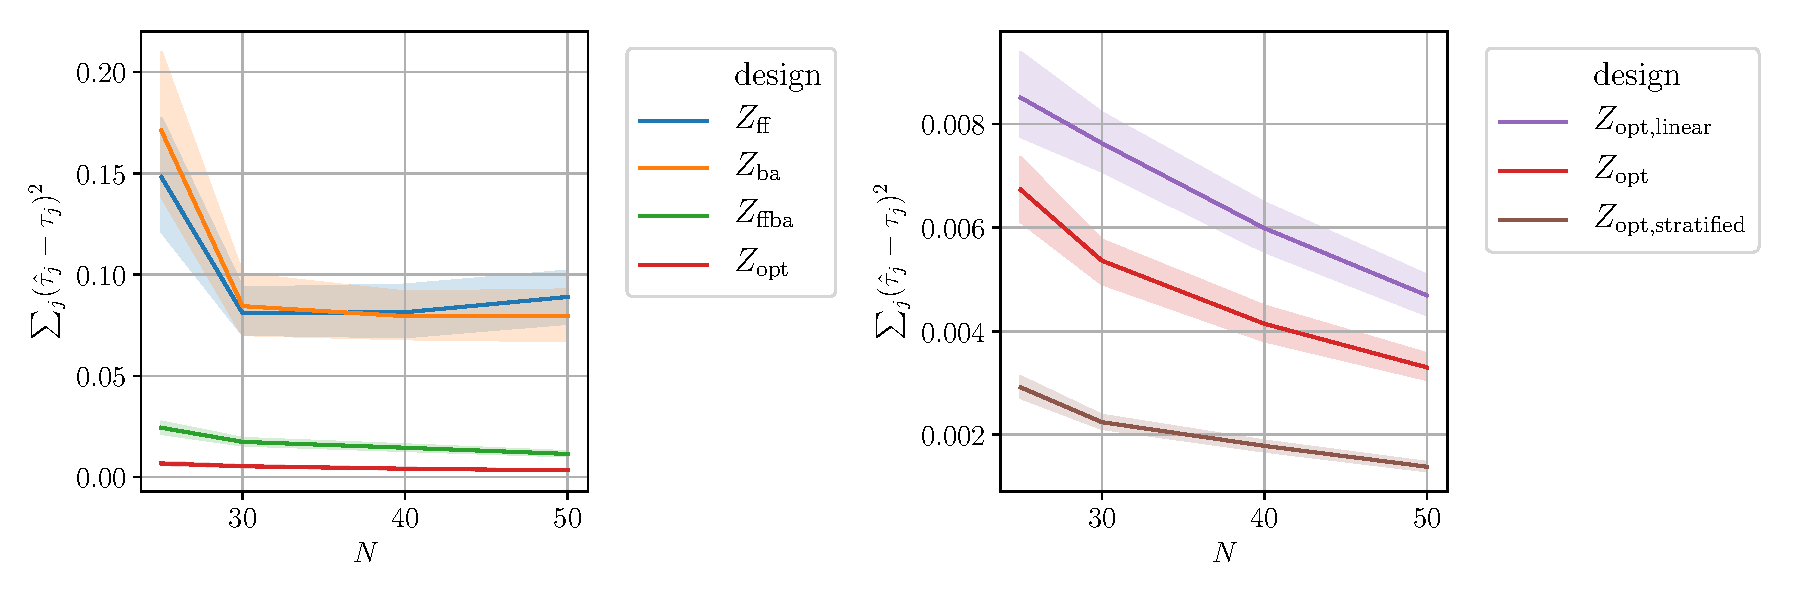
\includegraphics[width=0.8\linewidth]{plots/empirical/medical/medical_T_10_varying_N_lag_2_agg.pdf}
		\caption{Home medical visit data}
	\end{subfigure}
	\begin{subfigure}{1\textwidth}
		\centering
		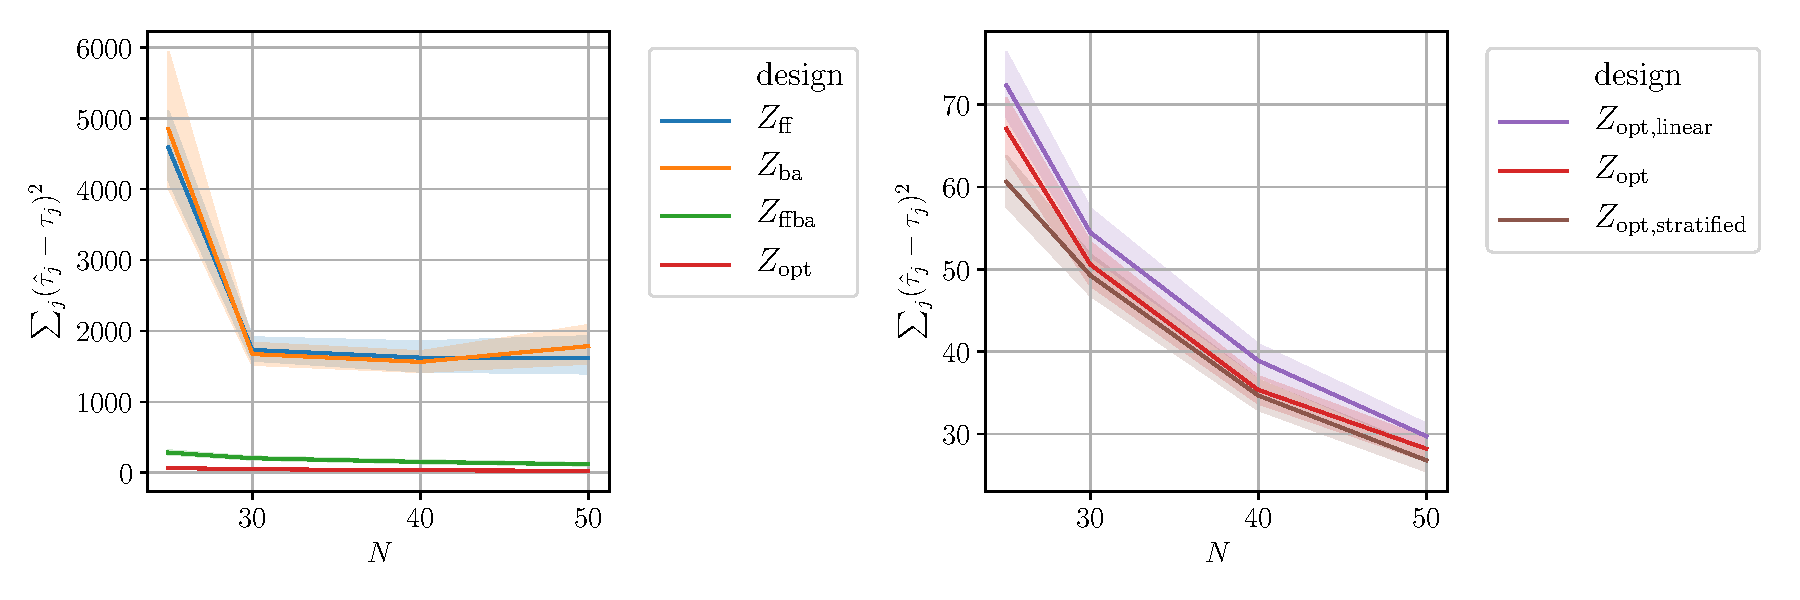
\includegraphics[width=0.8\linewidth]{plots/empirical/grocery/grocery_T_20_varying_N_lag_2_agg.pdf}
		\caption{Grocery data}
	\end{subfigure}
	\begin{subfigure}{1\textwidth}
		\centering
		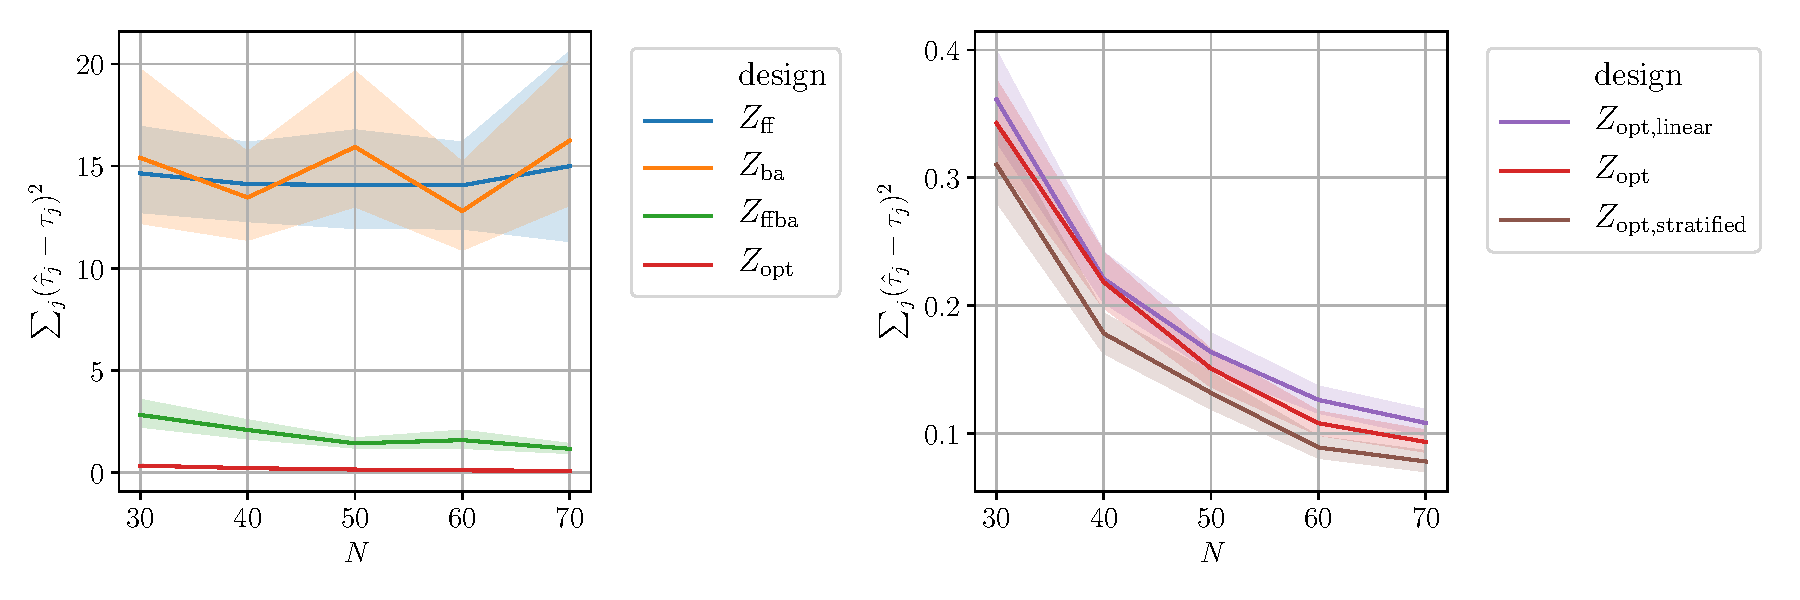
\includegraphics[width=0.8\linewidth]{plots/empirical/loan/loan_T_20_varying_N_lag_2_agg.pdf}
		\caption{Loan data}
	\end{subfigure}
	\caption{\textbf{Varying $N$ (additional data sets).} These figures show the mean and 95\% confidence band of $\sum_{j}(\hat{\tau}_j - \tau_j)^2$ for various designs, based on 2,000 synthetic non-adaptive experiments with $\ell = 2$ and varying $N$. For the medical data, $T$ is 10, and $\sum_{j= 0}^\ell \tau_j$ is $-10$\% of the average monthly visit rate. For the grocery data, $T$ is 20, and $\sum_{j= 0}^\ell \tau_j$ is $10$\% of the average weekly expenditure. For the loan data, $T$ is 20, and $\sum_{j= 0}^\ell \tau_j$ is $10$\% of the average monthly number of loans issued. The size of $\sum_{j= 0}^\ell \tau_j$ is for illustrative purpose, and the estimation error does not vary with the value of $\tau_j$ for all $j$.}
	\label{fig:additional-varying-N}
\end{figure}

\begin{figure}[H]
	\centering
	\begin{subfigure}{1\textwidth}
		\centering
		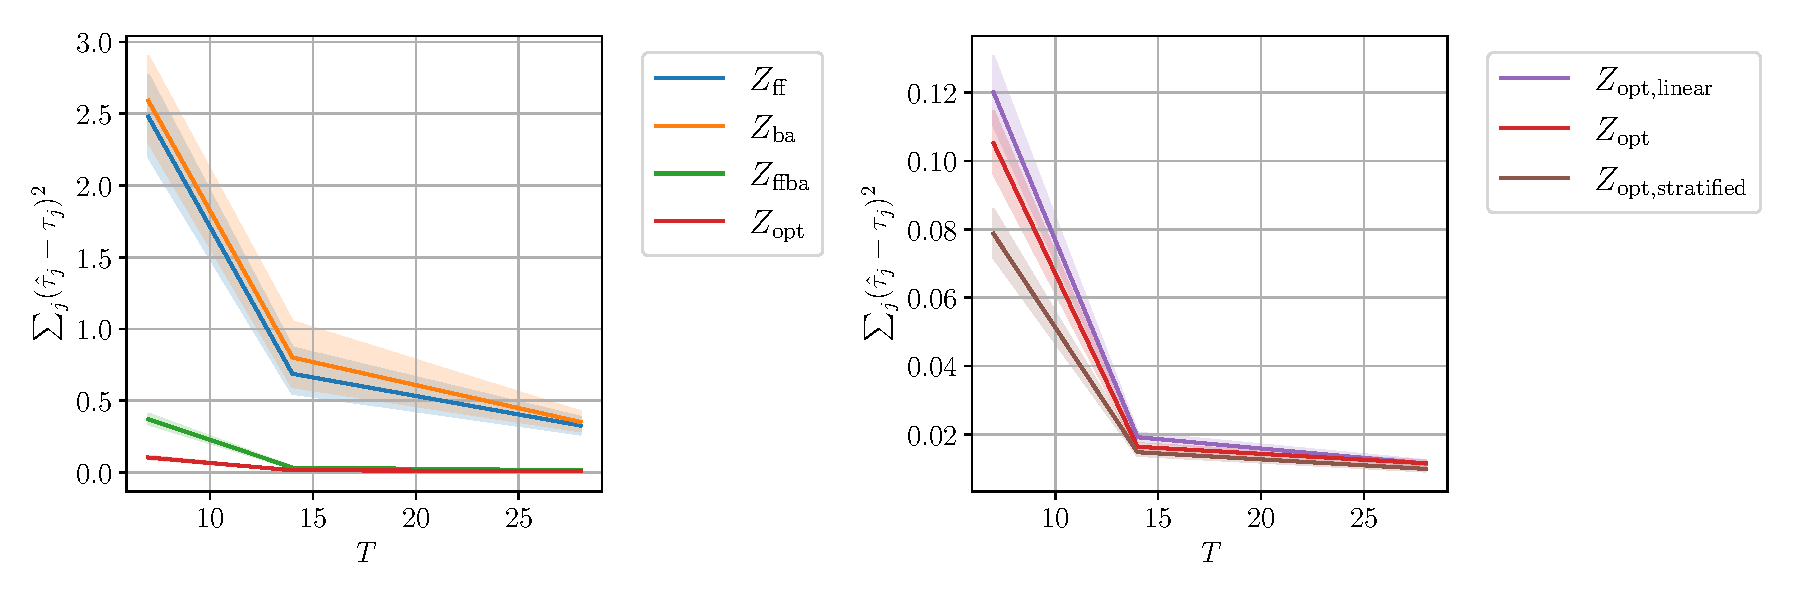
\includegraphics[width=0.75\linewidth]{plots/empirical/flu/nonadaptive/flu_N_50_varying_T_lag_2_agg.pdf}
		\caption{Flu data}
	\end{subfigure}
	\begin{subfigure}{1\textwidth}
		\centering
		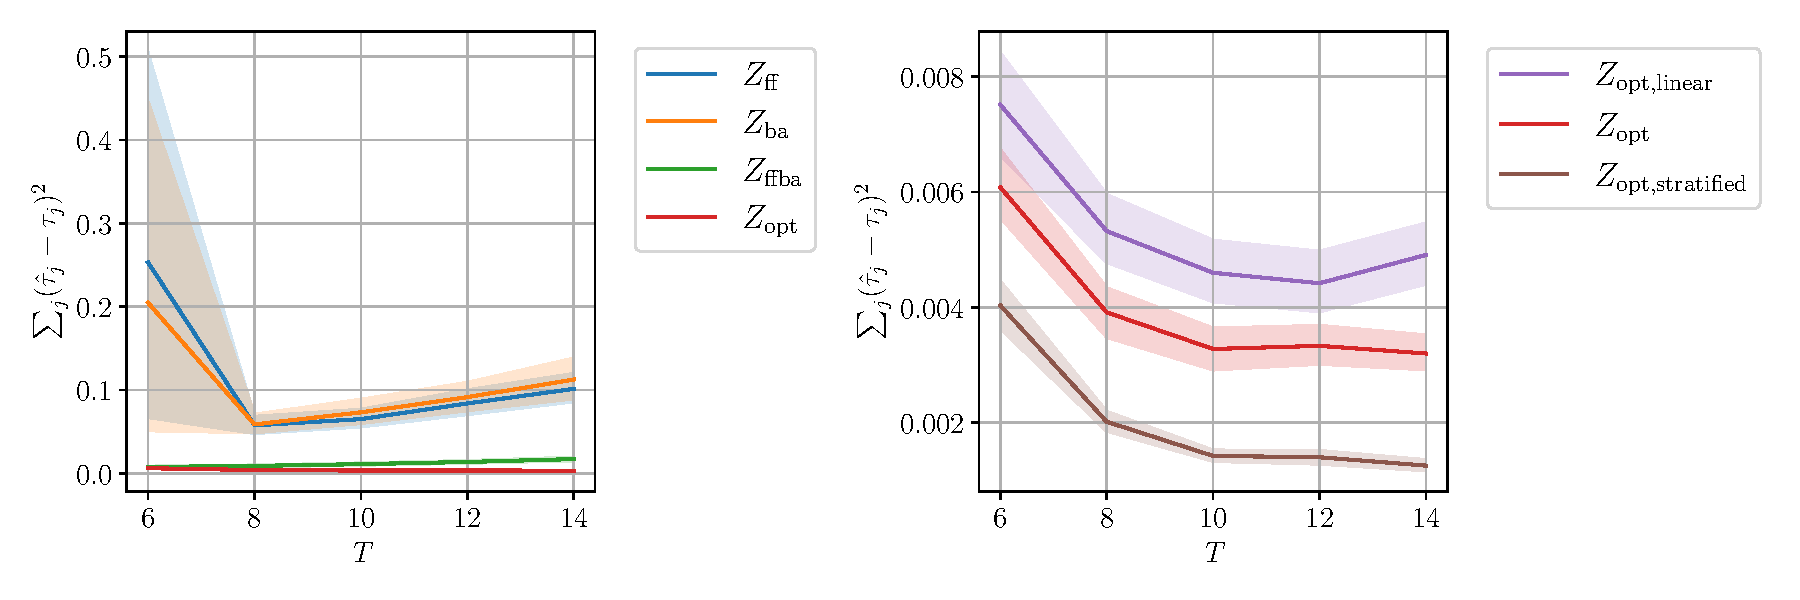
\includegraphics[width=0.75\linewidth]{plots/empirical/medical/medical_N_50_varying_T_lag_2_agg.pdf}
		\caption{Home medical visit data}
	\end{subfigure}
	\begin{subfigure}{1\textwidth}
		\centering
		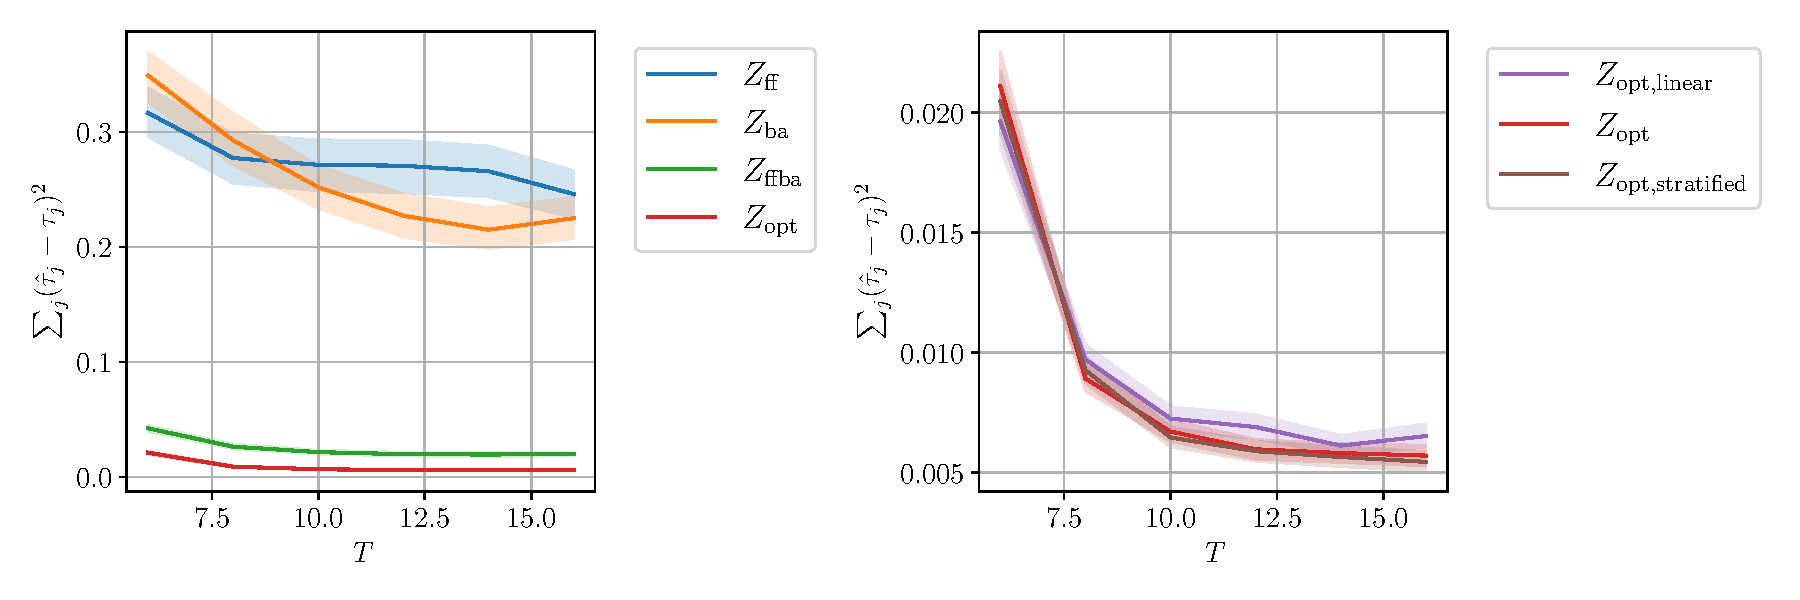
\includegraphics[width=0.75\linewidth]{plots/empirical/grocery/grocery_N_50_varying_T_lag_2_agg.pdf}
		\caption{Grocery data}
	\end{subfigure}
	\begin{subfigure}{1\textwidth}
		\centering
		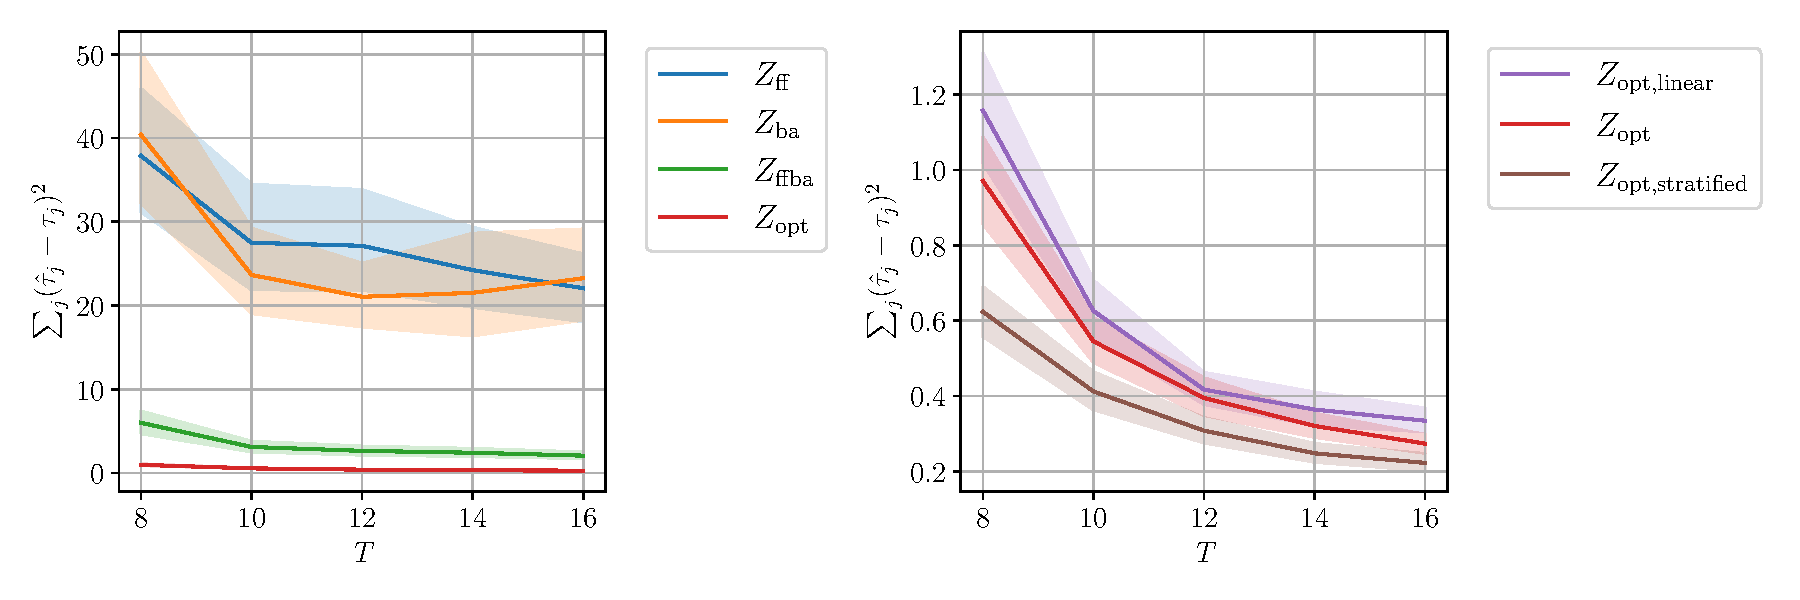
\includegraphics[width=0.75\linewidth]{plots/empirical/loan/loan_N_50_varying_T_lag_2_agg.pdf}
		\caption{Loan data}
	\end{subfigure}
	\caption{\textbf{Varying $T$.} These figures show the mean and 95\% confidence band of $\sum_{j}(\hat{\tau}_j - \tau_j)^2$ for various designs, based on 2,000 synthetic non-adaptive experiments with $\ell = 2$, $N = 50$, and varying $T$. The data generating process is identical to that in Figure \ref{fig:additional-varying-N}.}
	\label{fig:additional-varying-T}
\end{figure}
\clearpage

\subsubsection{Robustness to Specification of Estimator}\label{subsubsec:robustness-to-specification}

We compare the performance of various treatment designs, when the specification of the estimator varies:
%
\begin{itemize}
    \item ``no fe'': Least squares estimator of $\bm{\tau}$ using the specification $Y_{it} = c + \tau_0 z_{it} + \cdots + \tau_{\ell} z_{i,t-\ell} + \varepsilon_{it}$, which is the same as the difference-in-means estimator. 
    \item ``unit fe only'': Least squares estimator of $\bm{\tau}$ using the specification $Y_{it} = \alpha_i + \tau_0 z_{it} + \cdots + \tau_{\ell} z_{i,t-\ell} + \varepsilon_{it}$. 
    \item ``time fe only'': Least squares estimator of $\bm{\tau}$ using the specification $Y_{it} = \beta_t + \tau_0 z_{it} + \cdots + \tau_{\ell} z_{i,t-\ell} + \varepsilon_{it}$. 
    \item ``two-way fe'': Least squares estimator of  $\bm{\tau}$ using the specification $Y_{it} = \alpha_i + \beta_t +  \tau_0 z_{it} + \cdots + \tau_{\ell} z_{i,t-\ell} + \varepsilon_{it}$. (equivalent to the \within estimator of $\bm{\tau}$).
    \item ``two-way fe$+$covar'': Weighted least squares estimator of $\bm{\tau}$ using the specification \eqref{eqn:model-setup}, with $\*W \propto \big(\hat{\*U} \hat{\*\Sigma}_v \hat{\*U}^\T + \hat\sigma_\varepsilon^2 \*I_N \big)^\I$.
\end{itemize}

Figure \ref{fig:various-optimal-design} provides examples of T-optimal designs that maximize \eqref{eqn:obj} under each of the above five specifications. Figure \ref{fig:various-estimation-method} compares the total mean-squared error (MSE) of $\bm{\tau}$ of various designs under the above specifications of the estimator. Figure \ref{fig:bias-variance} decomposes the total MSE into bias squared and variance of various designs. There are three findings from Figure \ref{fig:various-estimation-method}:
%
\begin{enumerate}
    \item Allowing for time-fixed effects in the specification can significantly reduce MSE. The reduction mainly comes from bias reduction, and also comes from variance reduction for most designs. As the flu occurrence rate fluctuates by month, allowing for time-fixed effects can control this seasonality effect in the estimation of $\bm{\tau}$. This is particularly useful for estimation error reduction when $T$ is small (which is the case in this experiment).
    \item Allowing for covariates in the specification ({\it i.e.}, ``two-way fe$+$covar'') can further reduce MSE. The reduction mainly comes from variance reduction. 
    %
    \item 
    Among all the designs, $Z_{\mathrm{opt,linear}}$ and $Z_{\mathrm{opt,stratified}}$ have the smallest MSE and variance under various specifications. This implies that our designs are robust to specification of the the estimator (especially when misspecification is a concern).
\end{enumerate}
%
In summary, to maximally reduce the estimation error, both the treatment decisions (design) and the specification of estimator play major roles.

\begin{figure}[H]
	\centering
	\begin{subfigure}{.95\textwidth}
		\centering
		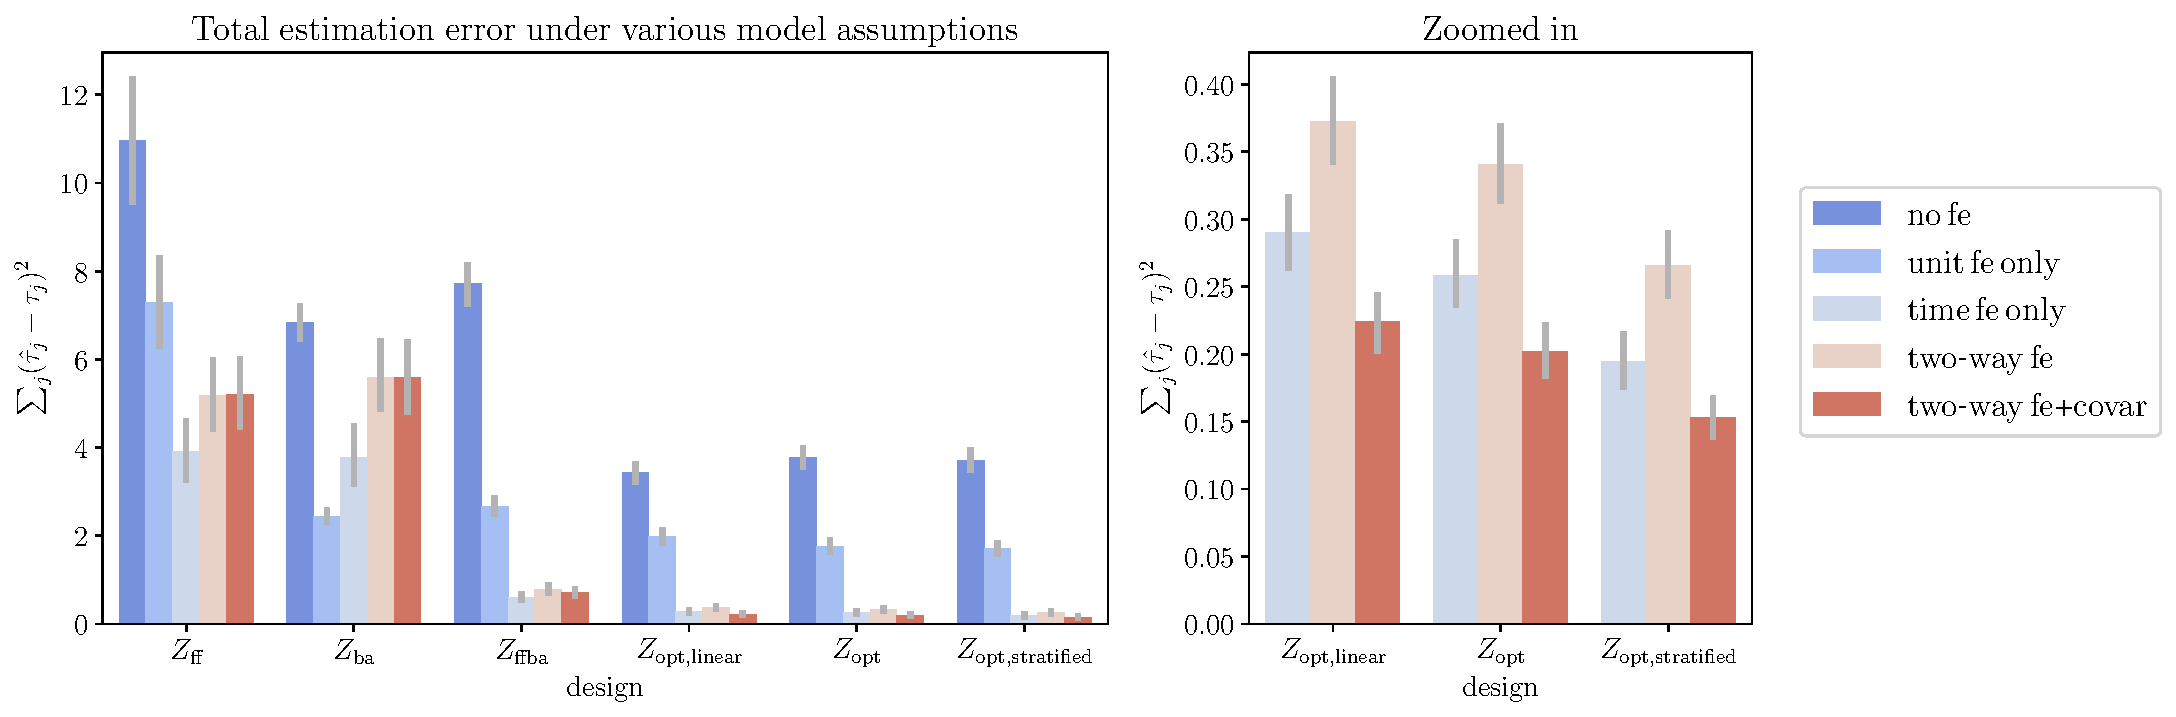
\includegraphics[width=1\linewidth]{plots/empirical/flu/nonadaptive/flu_N_25_T_7_various_methods-full.pdf}
	\end{subfigure}
	\caption{\textbf{Estimation error under various specifications.} Instantaneous and lagged effects are estimated under various specifications from 1,000 synthetic experiments of dimension $25\times 7$ with $\ell = 2$ on the flu data. }
	\label{fig:various-estimation-method}
\end{figure}


\begin{figure}[H]
	\centering
	\begin{subfigure}{.9\textwidth}
		\centering
		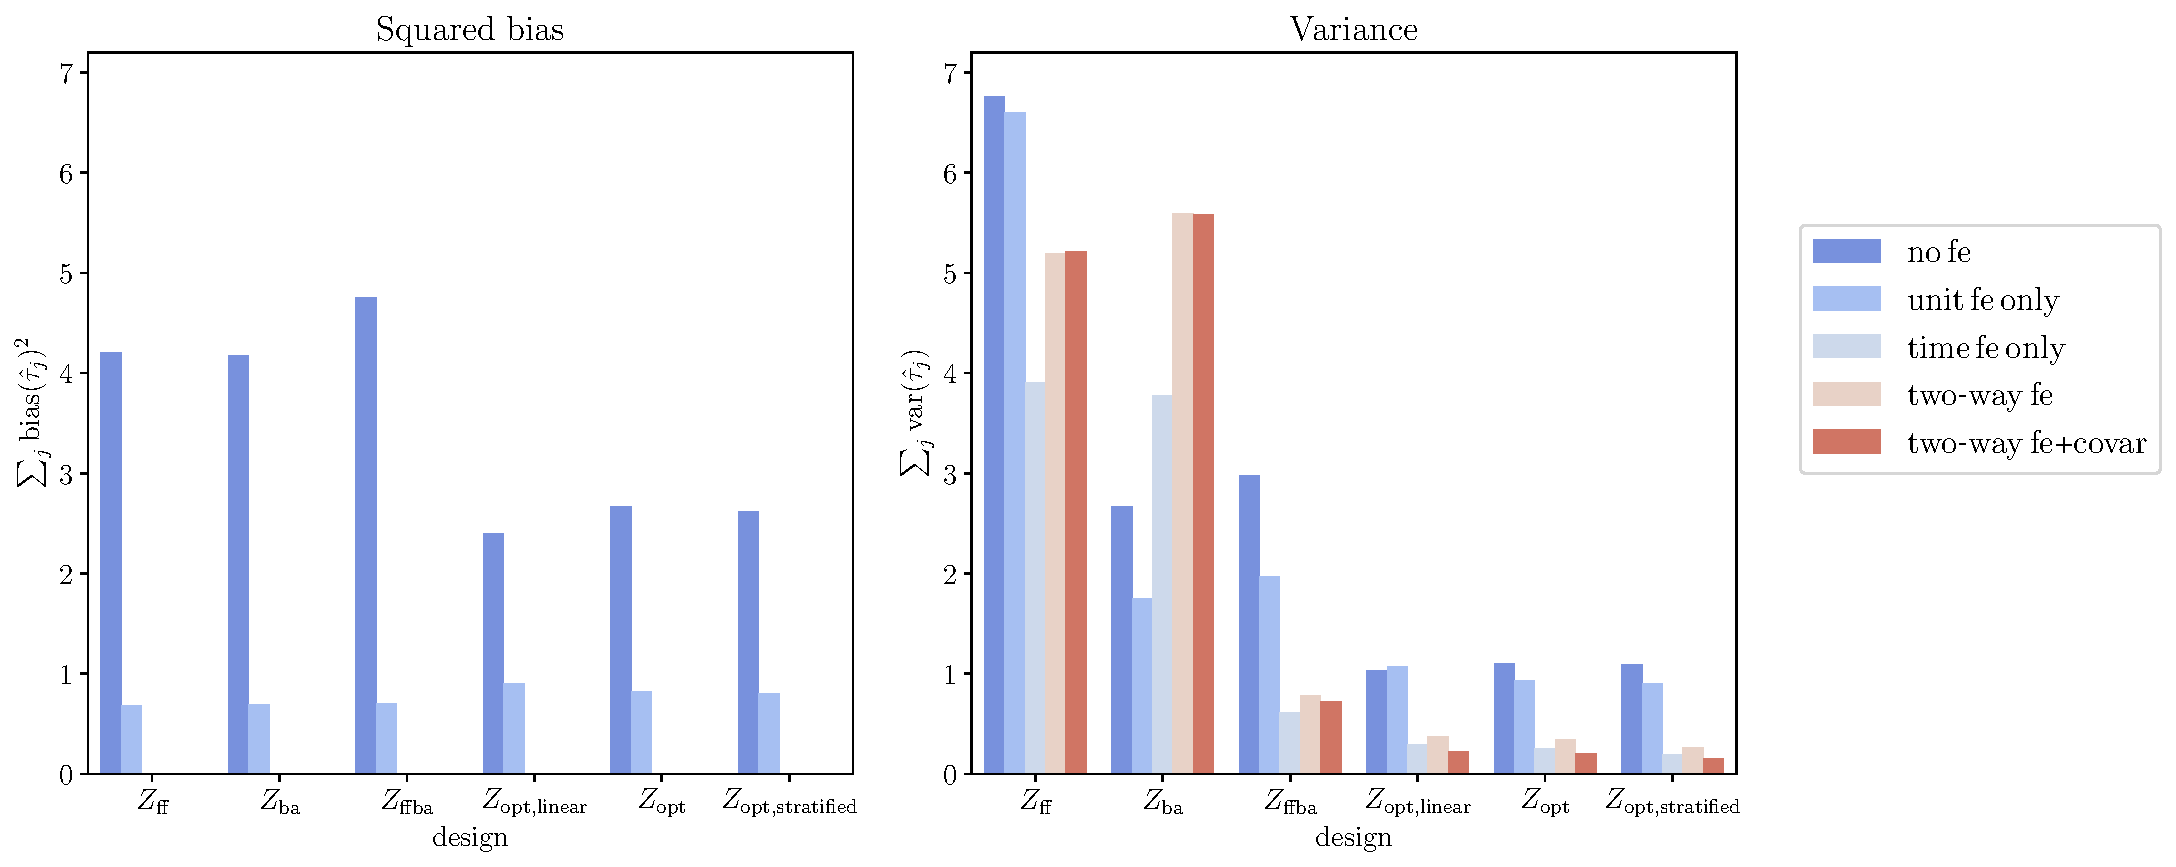
\includegraphics[width=1\linewidth]{plots/empirical/flu/nonadaptive/flu_N_25_T_7_bias-variance.pdf}
	\end{subfigure}
	\caption{\textbf{Bias and variance decomposition.} Instantaneous and lagged effects are estimated under various specifications from 1,000 synthetic experiments of dimension $25\times 7$ with $\ell = 2$ on the flu data. }
	\label{fig:bias-variance}
\end{figure}

% \clearpage

\subsubsection{Robustness to Alternative Metrics}\label{subsubsec:robustness-to-alternative-metrics}
We further evaluate various designs by alternative metrics. Specifically, we consider the squared estimation error of cumulative effect, that is, $\big(\sum_{j = 0}^{\ell} (\hat \tau_{j} - \tau_j) \big)^2$, and metrics related to hypothesis testing. When we conduct hypothesis testing, we are interested in true positives (TP), true negatives (TN), false positives (FP), and false negatives (FN) in the confusion matrix. For each $j \in \{0\} \cup [\ell]$, the positive class of $\tau_j$ is defined as $\{|\tau_j|=a\}$, and the negative class is defined as $\{|\tau_j|=0\}$. {\blue  We use the same $a$ for different $j$, so that the results of $\tau_j$ for different $j$ are comparable.\footnote{
In contrast to the estimation error metrics in which $\tau_j$'s are different, as $j$ varies, in the hypothesis testing metrics, they are all equal. However, we empirically confirm that varying $a$ does not change the ranking of the performance of various designs, with respect to the estimation error.
} }
On each randomly selected block from the original control data, we then run a pair of synthetic experiments such that $\tau_j$ is set to $a$ (positive class) in one experiment, or to $0$ (negative class) in the other experiment. We then calculate the ${\sf t}$-statistic of $\hat{\tau}_j$ for all of these $2m$ experiments: If the absolute ${\sf t}$-statistic is above some threshold $\iota$, the estimated class of $\tau_j$ is positive; otherwise, the estimated class is negative. We can then compare the true class with the estimated class on all $2m$ experiments, and count TP, TN, FP and FN for each $j$. If we vary the threshold $\iota$, in the same spirit as when the receiver operating characteristic (ROC) curve for a binary classification problem is generated, then the estimated class may change, and TP, TN, FP and FN may change as well. In fact, FP and FN are type I and type II errors of the test.
Therefore, we can vary $\iota$ and study, for various treatment designs, how the TP rate, or equivalently, power, varies with the FP rate, or equivalently, significance level. Similarly, we can study how the ``precision", $\mathrm{TP}/(\mathrm{TP}+\mathrm{FP})$, varies with the recall, $\mathrm{TP}/(\mathrm{TP}+\mathrm{FN})$.\footnote{We put ``precision" in quotes here to distinguish between this notion of ``precision" that is standard in statistical learning literature and our main precision metric defined in Section \ref{sec:model}.} Overall, for each $j$, $0\le j\le \ell$, we obtain one ROC curve and one ``precision"-recall curve.

The findings in Section \ref{subsec:fixed-sample-empirical-results} are robust to alternative evaluation metrics. Figure \ref{fig:varying-N-other-metrics} shows the squared estimation error of cumulative effect of various treatment designs on all four data sets. The findings from Figure \ref{fig:varying-N-other-metrics} are aligned with those from Figure \ref{fig:varying-N-flu}.
Figure \ref{fig:roc-equal-tau} shows the ROC curve of various designs (i.e., power vs. significance level) on the flu data for testing each of $\tau_0$, $\tau_1$, and $\tau_2$, for when significance level is up to 10\%. $Z_{\OPT,\mathrm{stratified}}$ has consistently higher power than all other designs, at all significance levels. $Z_{\OPT}$ also outperforms or nearly ties with $Z_{\OPT,\mathrm{linear}}$. These three of these designs dominate benchmarks ($Z_{\FF}$, $Z_{\BA}$, and $Z_{\FFBA}$). 
Their corresponding area under the curve (AUC) values (for the full ROC curves) are shown in 
Table \ref{tab:auc}. The AUC of $Z_{\FF}$ and $Z_{\BA}$ are consistently and significantly lower than the AUC of other treatment designs in the test of $\tau_0$, $\tau_1$ and $\tau_2$. The AUC of $Z_{\OPT}$ is consistently higher than that of $Z_{\FFBA}$ and the improvement is more noticeable for $\tau_1$. Consistent with the previous metric, $Z_{\OPT,\mathrm{stratified}}$ further improves upon $Z_{\OPT}$. 
\begin{figure}[h!]
\captionsetup{singlelinecheck = false, format= hang,justification=raggedright}
	\begin{subfigure}{0.286\textwidth}
		\centering
		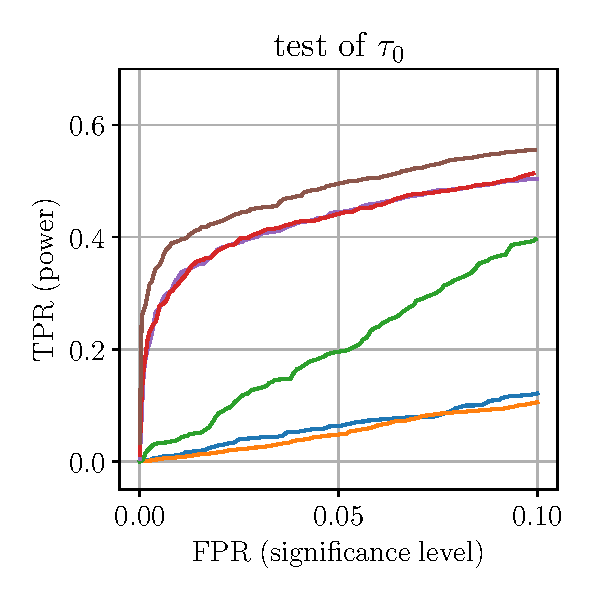
\includegraphics[width=1\linewidth]{plots/empirical/flu/nonadaptive/N_50_T_7_lag_2_-0.1_tau0_roc_equal_tau-line-plot.pdf}
	\end{subfigure}%
	\begin{subfigure}{0.286\textwidth}
		\centering
		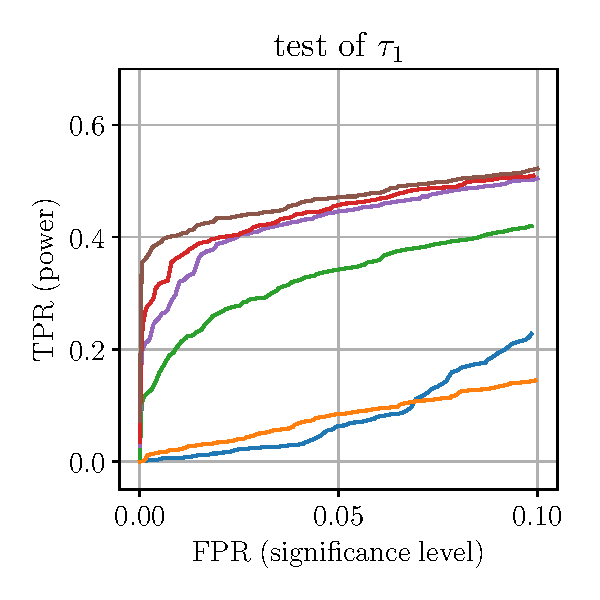
\includegraphics[width=1\linewidth]{plots/empirical/flu/nonadaptive/N_50_T_7_lag_2_-0.1_tau1_roc_equal_tau-line-plot.pdf}
	\end{subfigure}%
	\begin{subfigure}{0.429\textwidth}
		\centering
		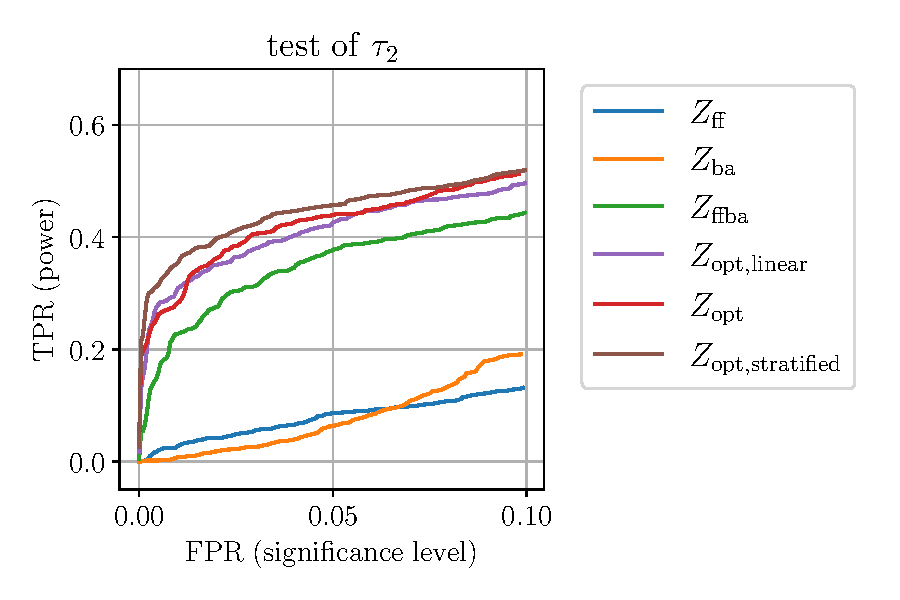
\includegraphics[width=1\linewidth]{plots/empirical/flu/nonadaptive/N_50_T_7_lag_2_-0.1_tau2_roc_equal_tau-line-plot.pdf}
	\end{subfigure}
	\caption{\textbf{ROC curve.} The TP and FP rates are calculated from 2,000 pairs of synthetic experiments with dimension $50\times 7$ and $\ell = 2$ on the flu data. The true positive class of $\tau_j$ is defined as $\{|\tau_j| = 0.1(NT)^{-1} \sum_{i,t} Y_{it}(-\bm{1}_{\ell+1})\}$. }
	\label{fig:roc-equal-tau}
\end{figure}

\begin{table}[h!]
    \centering
    {
    \begin{tabular}{l|p{1.5cm}p{1.5cm}p{1.5cm}p{1.5cm}p{1.5cm}p{1.8cm}}
\toprule
 &  $Z_{\FF}$ &  $Z_{\BA}$ &  $Z_{\FFBA}$ &  $Z_{\OPT}$ &  $Z_{\OPT,\mathrm{linear}}$ &  $Z_{\OPT,\mathrm{stratified}}$  \\
\midrule
$\tau_0$   &              0.614 &              0.633 &                0.744 &               0.750 &                      0.740 &                          0.761 \\
$\tau_1$   &              0.598 &              0.563 &                0.702 &               0.745 &                      0.740 &                          0.756 \\
$\tau_2$   &              0.590 &              0.629 &                0.738 &               0.748 &                      0.736 &                          0.762 \\
\bottomrule
\end{tabular}
    }
    \caption{\textbf{AUC.} AUC of various treatment designs and hypothesis tests in Figure \ref{fig:roc-equal-tau}.}
    \label{tab:auc}
\end{table}

\clearpage

\begin{figure}[H]
	\centering
	\begin{subfigure}{1\textwidth}
		\centering
		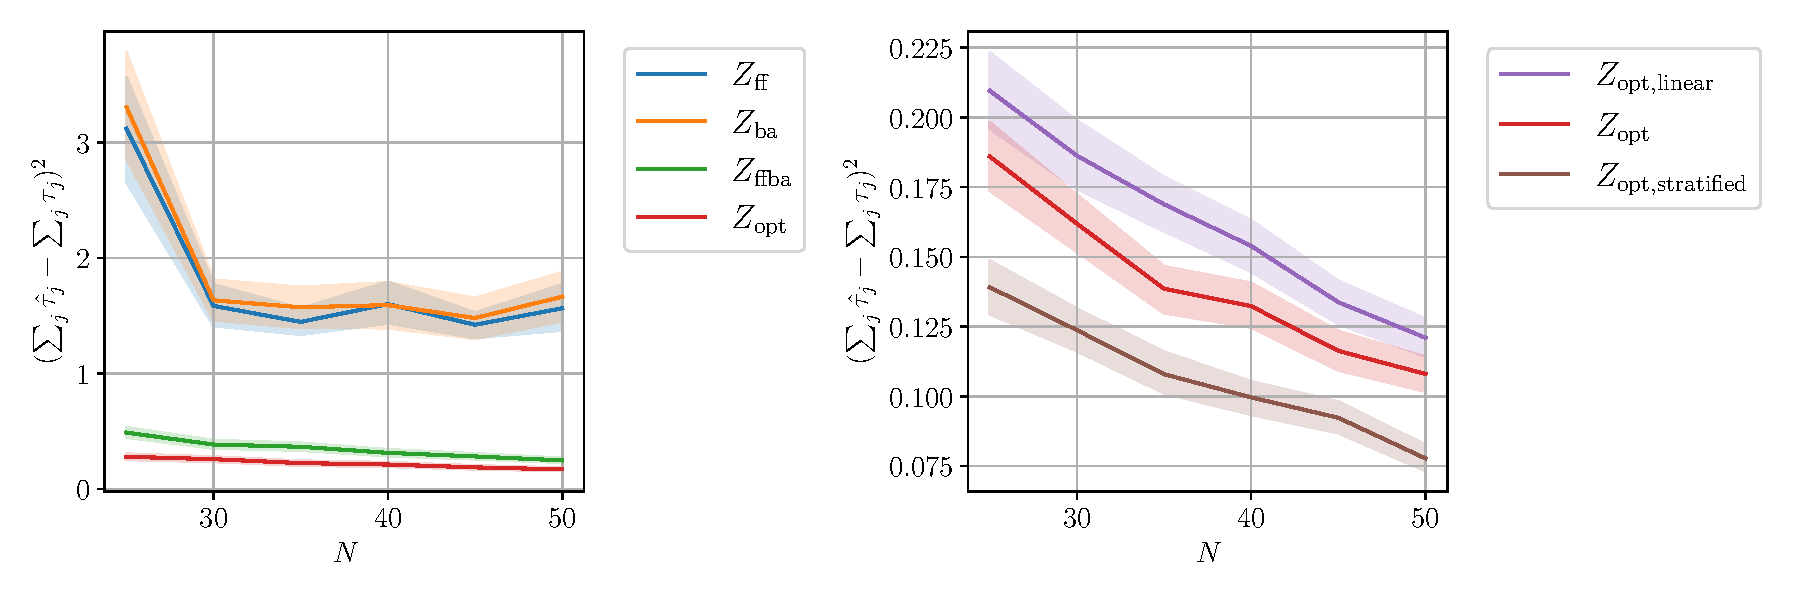
\includegraphics[width=0.65\linewidth]{plots/empirical/flu/nonadaptive/flu_T_7_varying_N_lag_2_total-effect.pdf}
		\caption{Flu data}
	\end{subfigure}
	\begin{subfigure}{1\textwidth}
		\centering
		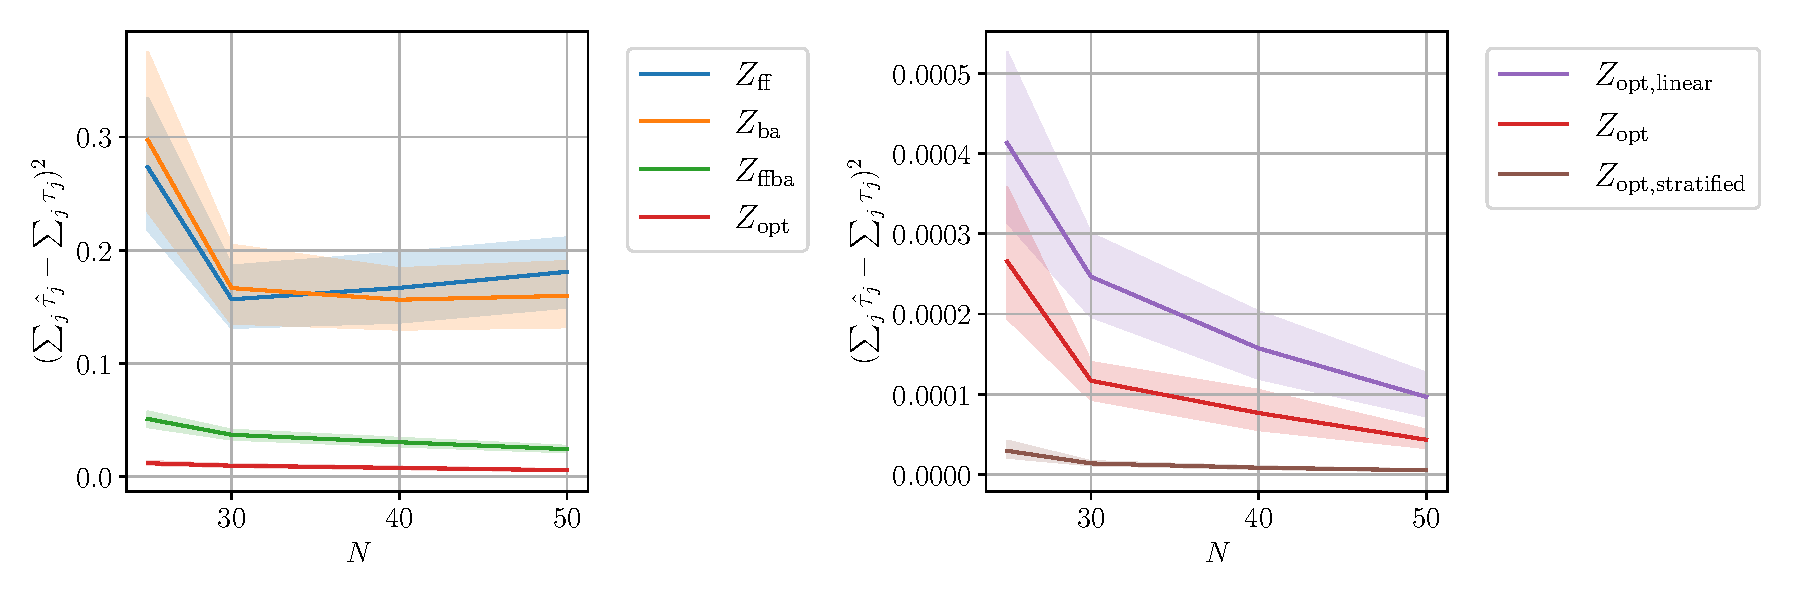
\includegraphics[width=0.65\linewidth]{plots/empirical/medical/medical_T_10_varying_N_lag_2_total-effect.pdf}
		\caption{Home medical visit data}
	\end{subfigure}
	\begin{subfigure}{1\textwidth}
		\centering
		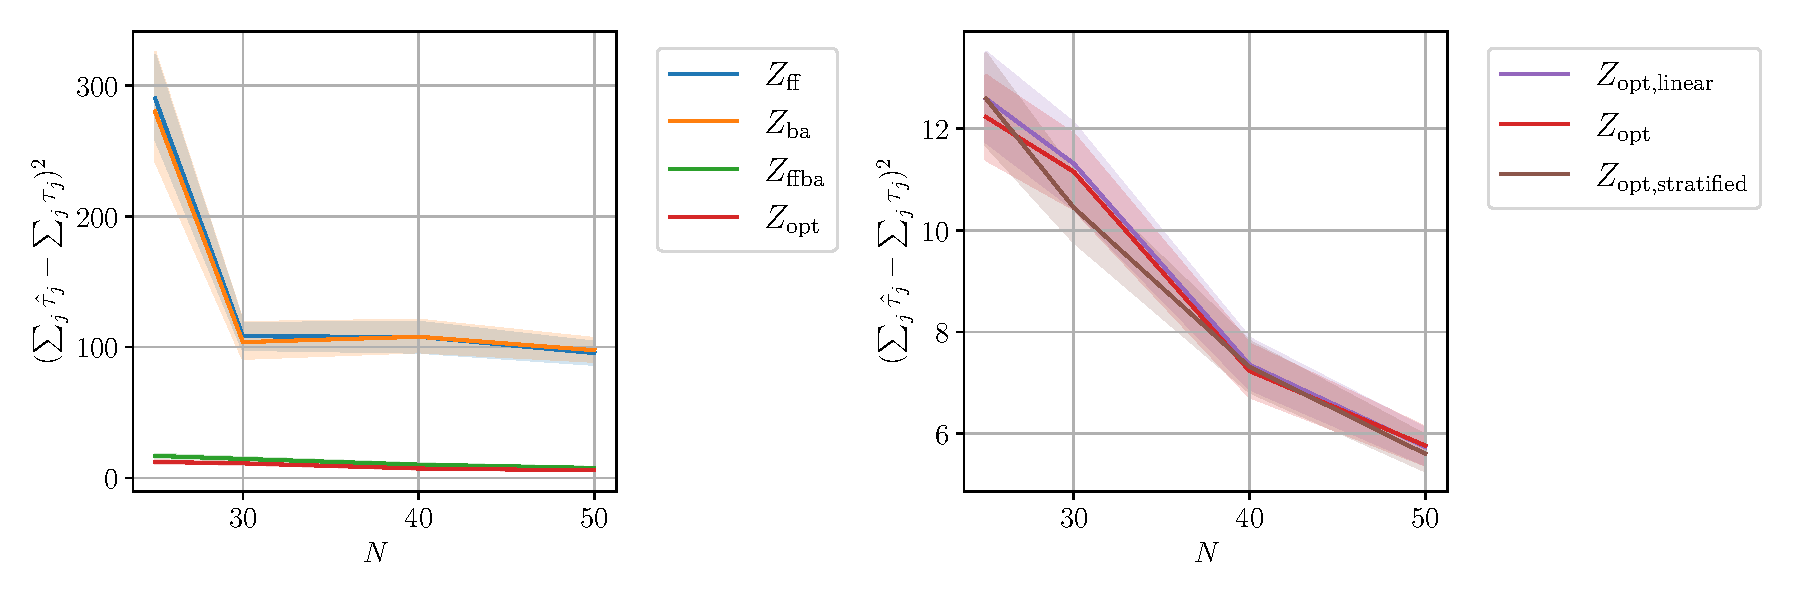
\includegraphics[width=0.65\linewidth]{plots/empirical/grocery/grocery_T_20_varying_N_lag_2_total-effect.pdf}
		\caption{Grocery data}
	\end{subfigure}
	\begin{subfigure}{1\textwidth}
		\centering
		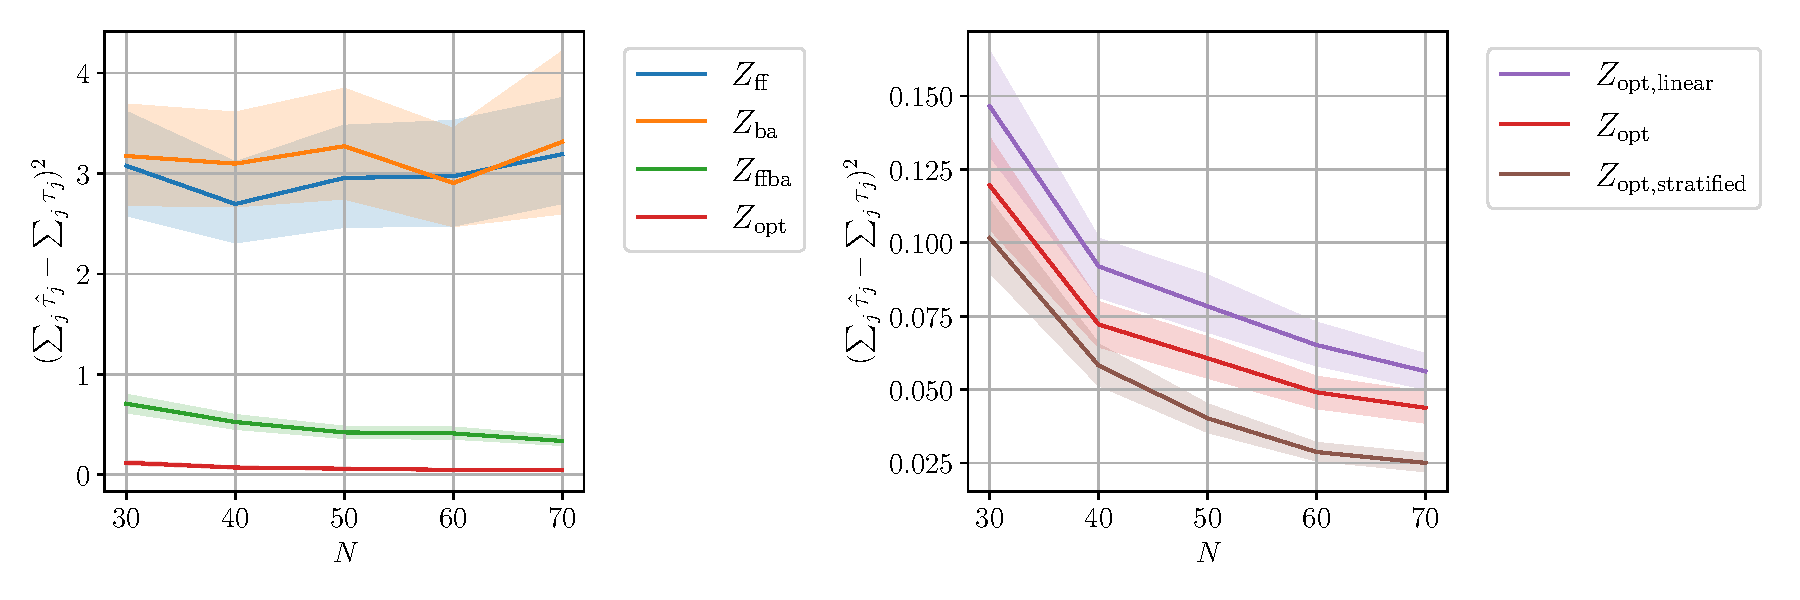
\includegraphics[width=0.65\linewidth]{plots/empirical/loan/loan_T_20_varying_N_lag_2_total-effect.pdf}
		\caption{Loan data}
	\end{subfigure}
	\vspace{0.05in}
	\caption{\textbf{Alternative metrics: squared estimation error of cumulative effect.} These figures show the mean and 95\% confidence band of the squared estimation error of the cumulative effect of various designs, based on 2,000 randomly sampled blocks with $\ell = 2$. The data generating process is identical to that in Figure \ref{fig:additional-varying-N}.}
	\label{fig:varying-N-other-metrics}
\end{figure}
\clearpage

\subsubsection{Varying Treatment Effects.}\label{subsubsec:magnitude-treatment-effect}

The total estimation error does not vary with the magnitude of treatment effects, as shown in Figure \ref{fig:varying-effect}. This is because the (weighted) least squares estimator is linear $Y_{it}$, and $Y_{it}$ is specified as linear in $\bm{\tau}$. Therefore, the estimation error of the (weighted) least squares estimator can be written as a linear function of residuals $\varepsilon_{it}$ that does not depend on $\bm{\tau}$, implying that the estimation error does not depend on the magnitude of treatment effects. 

Furthermore, we compare various designs when the treatment only has the instantaneous effect in Figure \ref{fig:instantaneous-effect}. In this case, the treated fractions in $Z_{\OPT,\mathrm{linear}}$ and $Z_{\OPT,\mathrm{stratified}}$ are optimal, but the treated fractions in $Z_{\OPT,\mathrm{nonlinear}}$ are sub-optimal. $Z_{\OPT,\mathrm{stratified}}$, as the stratified version of $Z_{\OPT,\mathrm{linear}}$, has lowest error among all designs.

\begin{figure}[H]
	\centering
	\begin{subfigure}{1\textwidth}
		\centering
		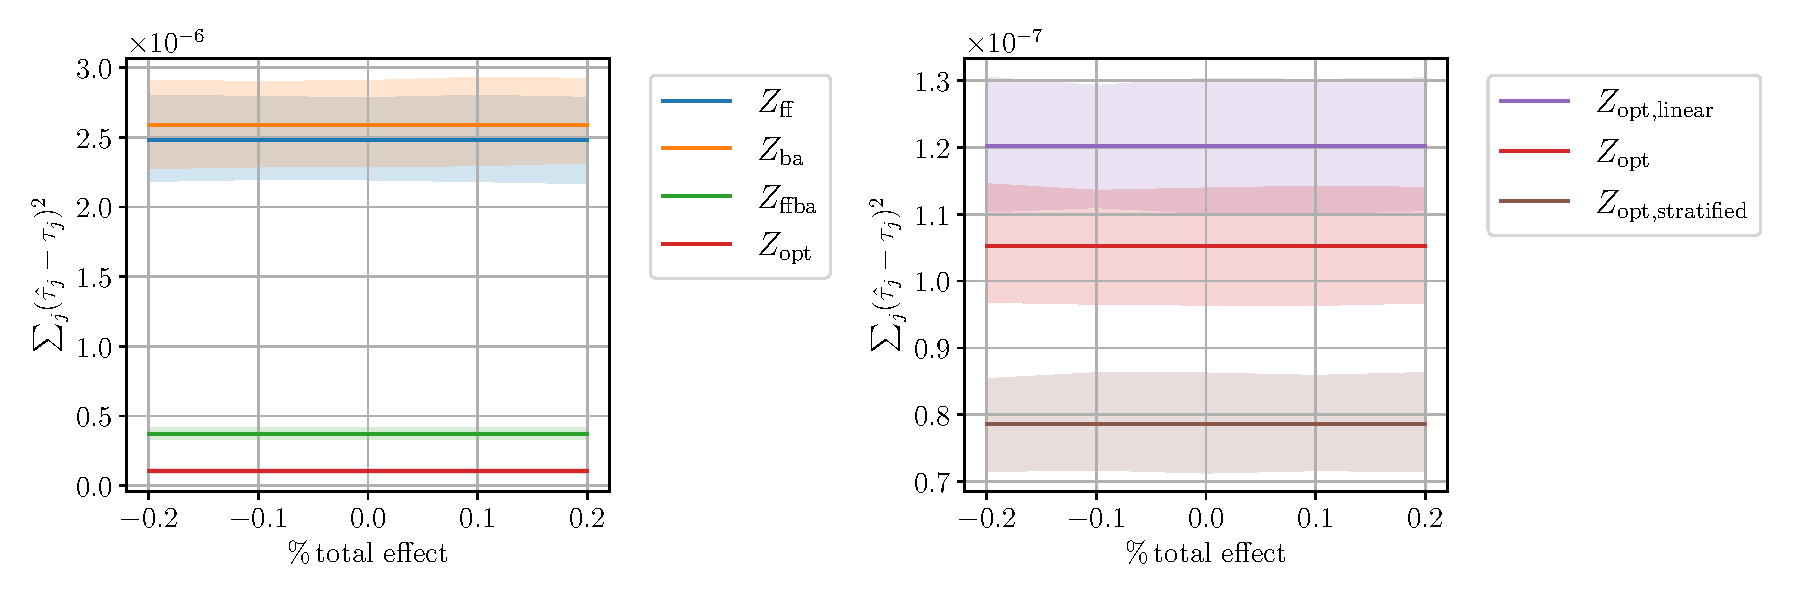
\includegraphics[width=0.75\linewidth]{plots/empirical/flu/nonadaptive/flu_N_50_T_7_varying_treatment_effect_lag_2_agg.pdf}
% 		\caption{Flu data}
	\end{subfigure}
	\vspace{0.01in}
	\caption{\textbf{Varying magnitude of treatment effects.} These figures show the mean and 95\% confidence band of $\sum_{j}(\hat{\tau}_j - \tau_j)^2$ for various designs, based on 1,000 synthetic non-adaptive experiments with $\ell = 2$, $T = 7$ and $N = 50$ on the flu data. The red curve in two figures are identical. The right figure zooms in the left one. The total cumulative effect varies from $-20$\% to $20$\% of the average monthly flu occurrence rate. The total estimation error stays constant with varying total cumulative effect.}
	\label{fig:varying-effect}
\end{figure}

\subsubsection{Varying duration of carryover effects $\ell$}\label{ecsub:varying-ell}

\begin{figure}[H]
	\centering
	\begin{subfigure}{1\textwidth}
		\centering
		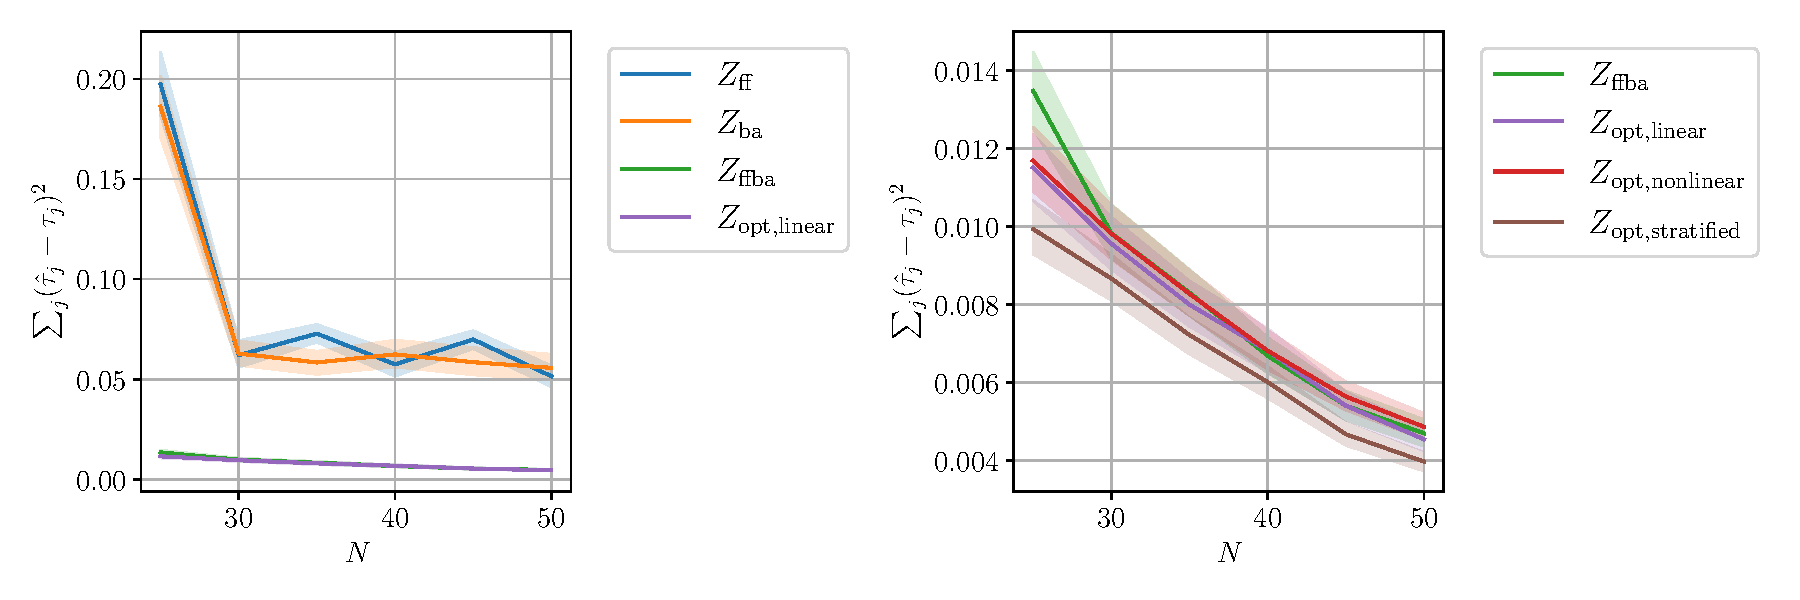
\includegraphics[width=0.75\linewidth]{plots/empirical/flu/nonadaptive/flu_T_14_varying_N_lag_0_agg-2.pdf}
% 		\caption{Flu data}
	\end{subfigure}
	\caption{\textbf{Instantaneous effect only.} 
 These figures show the mean and 95\% confidence band of $(\hat{\tau}_0 - \tau_0)^2$ for various designs, based on 1,000 synthetic non-adaptive experiments with $\ell = 0$, $T = 14$ and varying $N$. The red curve in two figures are identical. The right figure zooms in the left one. The instantaneous effect equals $-10$\% of the average monthly flu occurrence rate. }
	\label{fig:instantaneous-effect}
\end{figure}



\subsubsection{Specification of $\ell$}\label{ecsec:spec-ell}

Figure \ref{fig:varying-ell} shows the estimation error under various specifications of $\ell$. The bias of $\hat{\bm{\tau}}$ generally decreases with $\ell$ when $\ell$ is smaller than the true $\ell$. However, the variance of $\hat{\bm{\tau}}$ generally increases with $\ell$. When $\ell$ is correctly specified, the estimation error of $\hat{\bm{\tau}}$ is the lowest, as compared to other specifications of $\ell$, for all treatment designs. 

\begin{figure}[H]
	\centering
	\begin{subfigure}{1.0\textwidth}
		\centering
		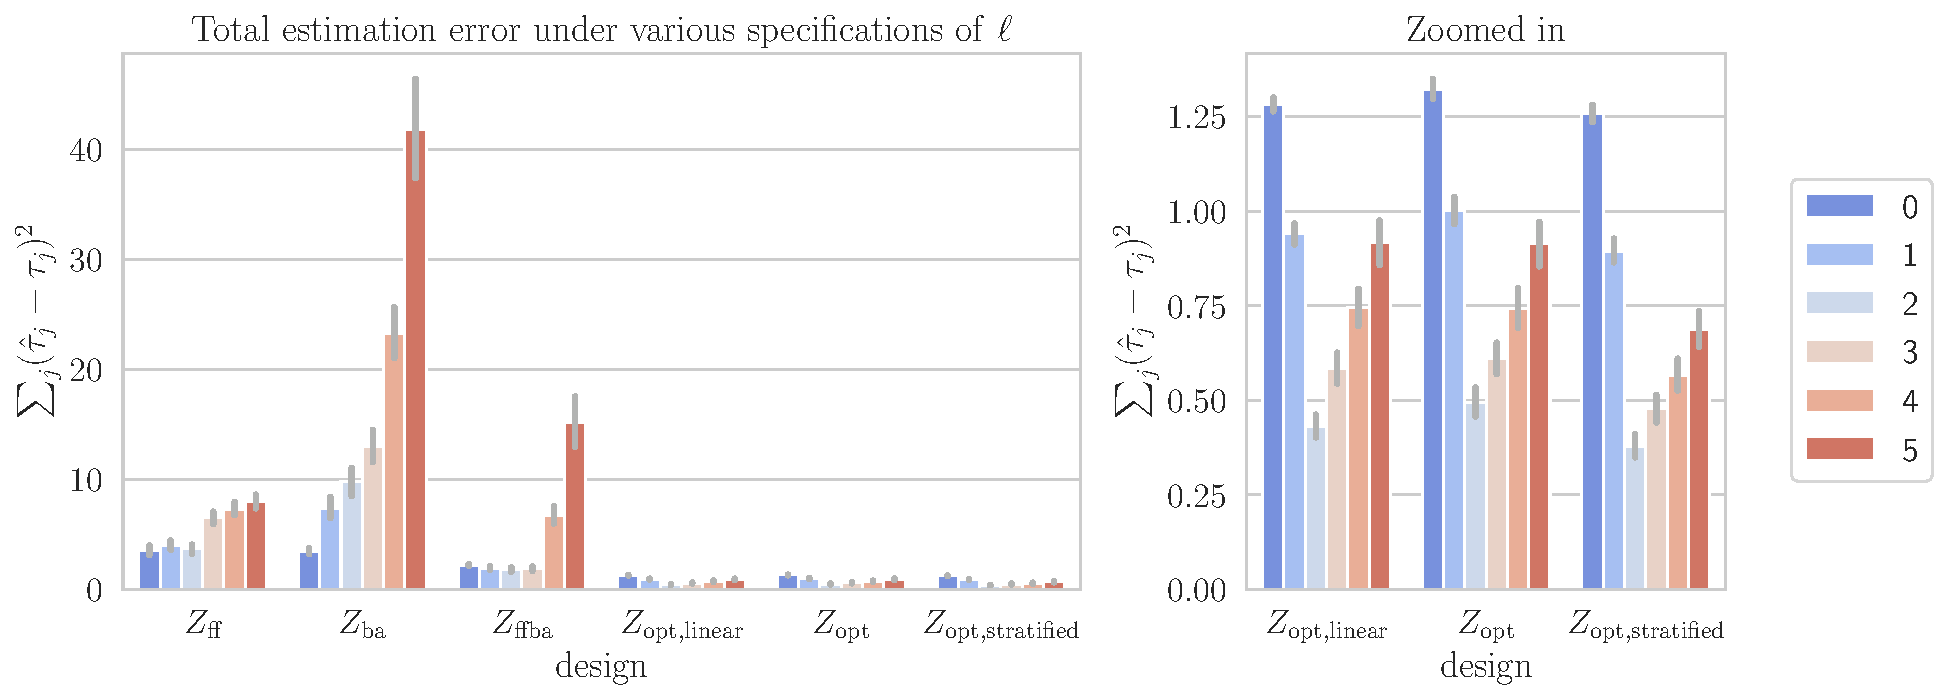
\includegraphics[width=1\linewidth]{plots/empirical/flu/nonadaptive/flu_N_50_T_7_varying-ell.pdf}
% 		\caption{Flu data}
	\end{subfigure}
	%\vspace{0.001in}
	\caption{\textbf{Varying $\ell$.} Instantaneous and lagged effects are estimated under various specifications of $\ell$ from 1,000 synthetic experiments of dimension $50\times 7$ with the true number of lags as $2$ on the flu data. The model assumptions are identical to those in Figure \ref{fig:various-optimal-design}.}
	\label{fig:varying-ell}
\end{figure}




% \clearpage
\subsection{Supplementary Results for Adaptive Experiments}

The results in Section \ref{subsec:sequential-result} are robust to the choice of experiment termination threshold $c$, as shown by the histograms of experiment termination times in Figure \ref{fig:experiment-termination-time-supp} and the estimation errors of various designs in Figure \ref{fig:various-opt-design-supp}. In addition, by comparing Figure \ref{fig:experiment-termination-time} with Figure \ref{fig:experiment-termination-time-supp}, the experiment termination times tend to increase with the threshold $c$, which is as expected. Moreover, by comparing Figure \ref{fig:various-opt-design} and Figure \ref{fig:various-opt-design-supp}, the estimation errors tend to increase with the threshold $c$ for all designs, which is also as expected.




    \begin{figure}[h!]
    \centering
    \begin{subfigure}{1\textwidth}
		\centering
		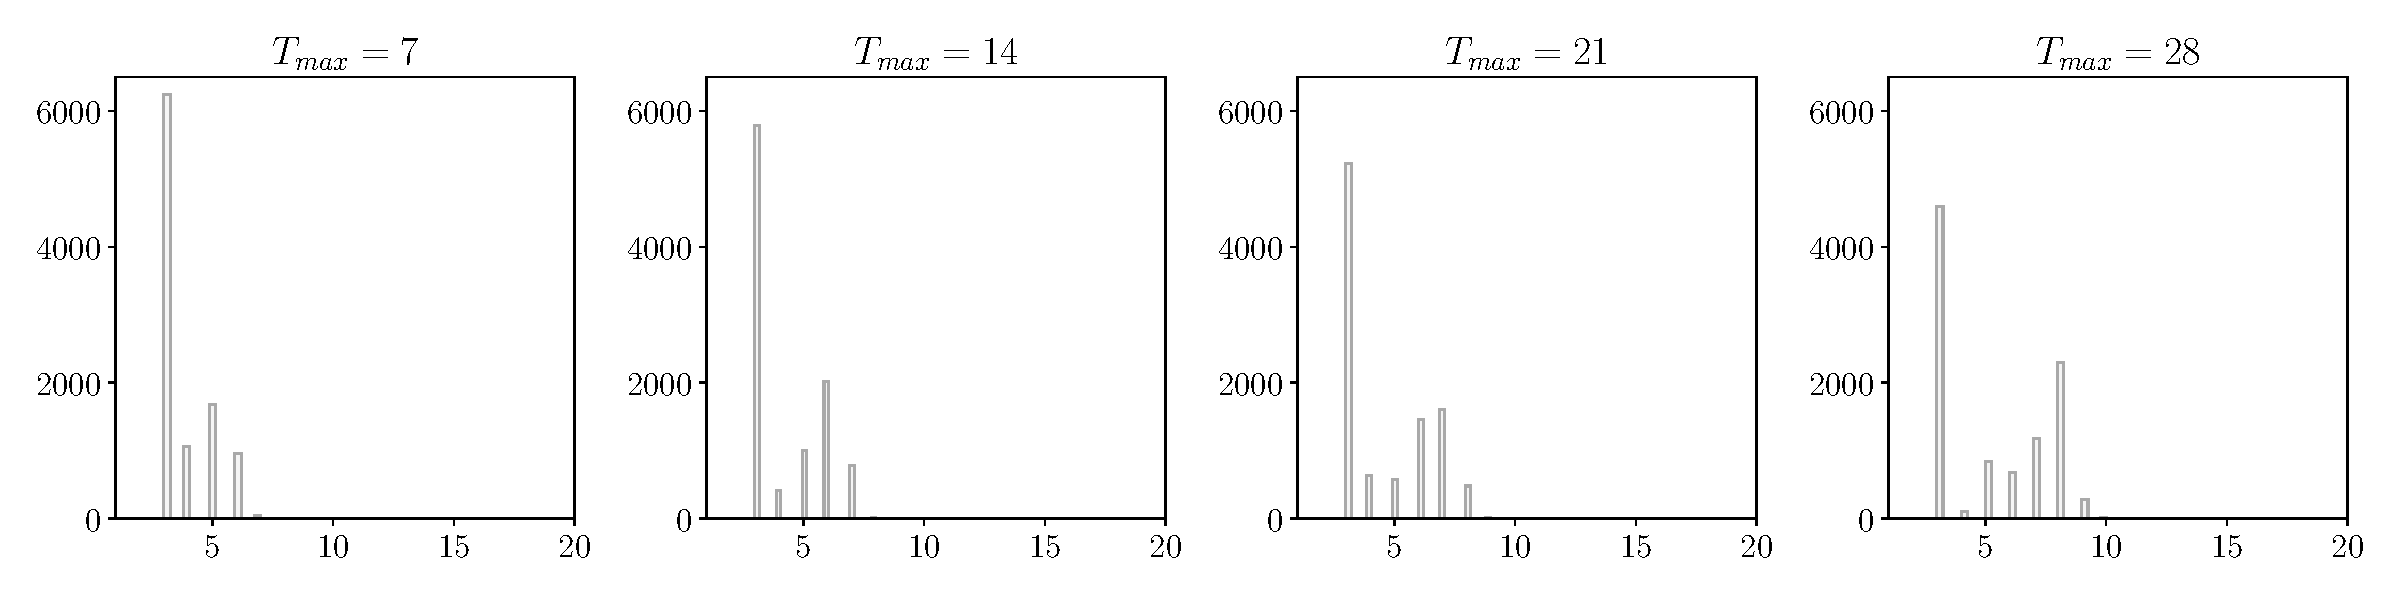
\includegraphics[width=1\linewidth]{plots/empirical/flu/adaptive/flu_termination_time-10.pdf}
		\caption{small threshold $c = 0.01 \cdot N/\tau_0^2$}
	\end{subfigure}
	\begin{subfigure}{1\textwidth}
		\centering
		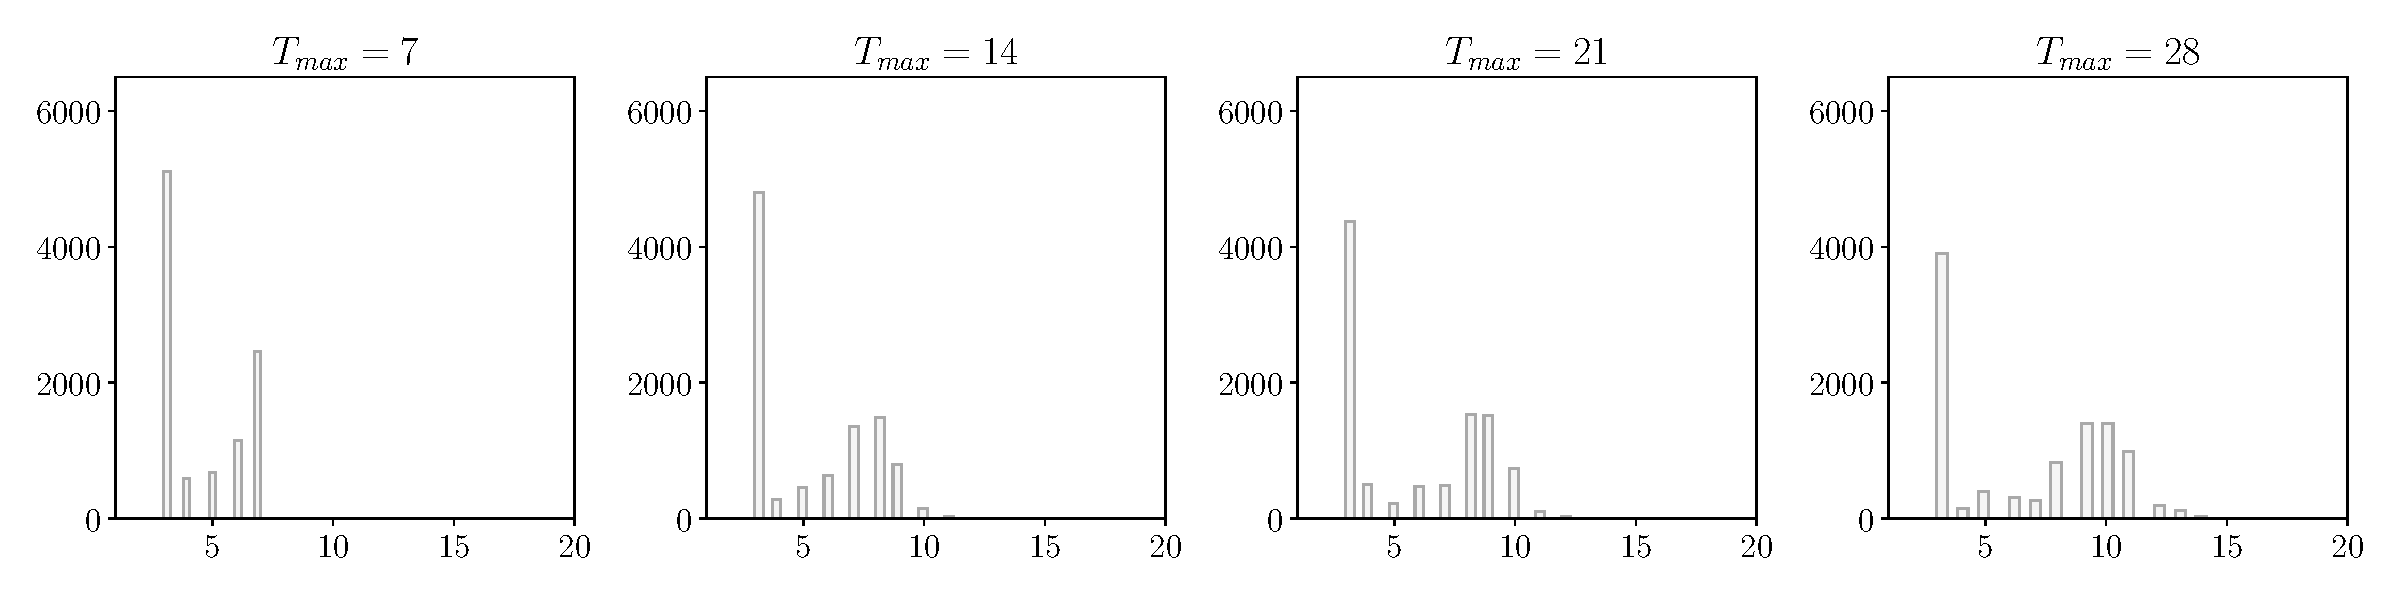
\includegraphics[width=1\linewidth]{plots/empirical/flu/adaptive/flu_termination_time-20.pdf}
		\caption{large threshold $c = 0.02 \cdot N/\tau_0^2$}
	\end{subfigure}
	\smallskip
	\caption{\textbf{Empirical distribution of termination time $\tilde{T}$ with alternative thresholds} This figure shows the histogram of the termination time $\tilde{T}$ for $T_{\max} \in \{7,14,21,28\}$ based on 10,000 sequential experiments. $N$ is chosen at $50$. In PGAE, the set of NTU has $N p_{\fcs} = 50 \times 0.2 = 10$ units, and both first and second sets of ATU has $N p_{\ad,1} =N p_{\ad,2} =  50 \times 0.4 = 20$ units.  $\tau_0$ is chosen at $/{-0.1}/{(NT_{\max})} \sum_{i,t} Y_{it}(-1)$ (i.e., 10\% of the average monthly flu occurrence rate). The earliest termination time $t_0$ is set as $3$. 
	}
	\label{fig:experiment-termination-time-supp}
\end{figure}


    \begin{figure}[h!]
    \centering
    \begin{subfigure}{0.5\textwidth}
		\centering
		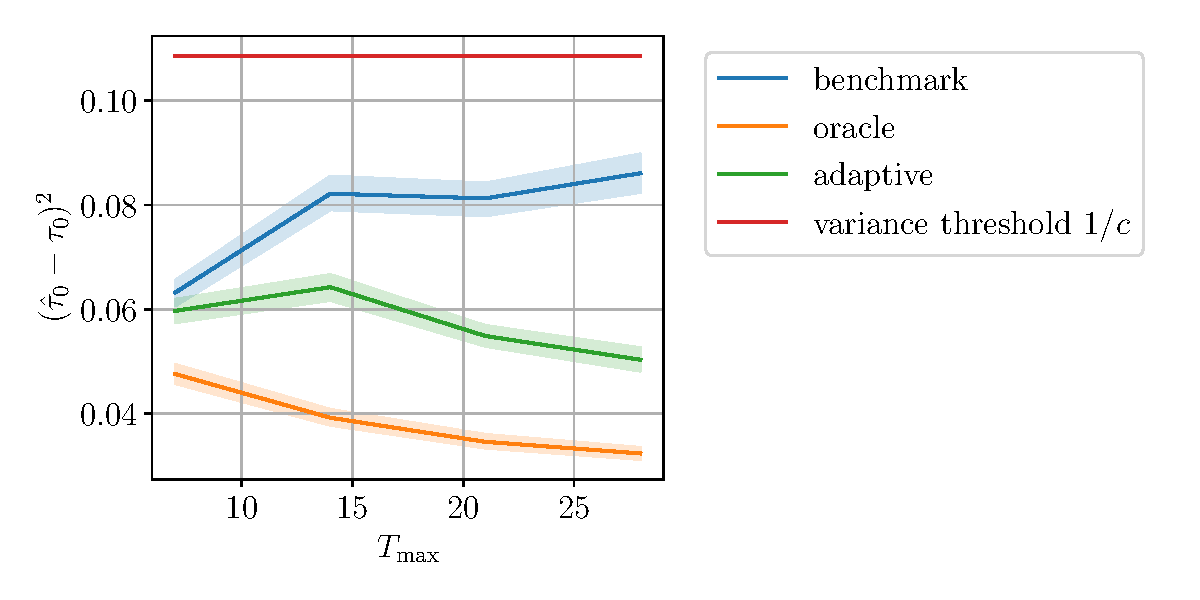
\includegraphics[width=1\linewidth]{plots/empirical/flu/adaptive/flu_adaptive_comparison-10.pdf}
		\caption{small threshold $c = 0.01 \cdot N/\tau_0^2$}
	\end{subfigure}%
	\begin{subfigure}{0.5\textwidth}
		\centering
		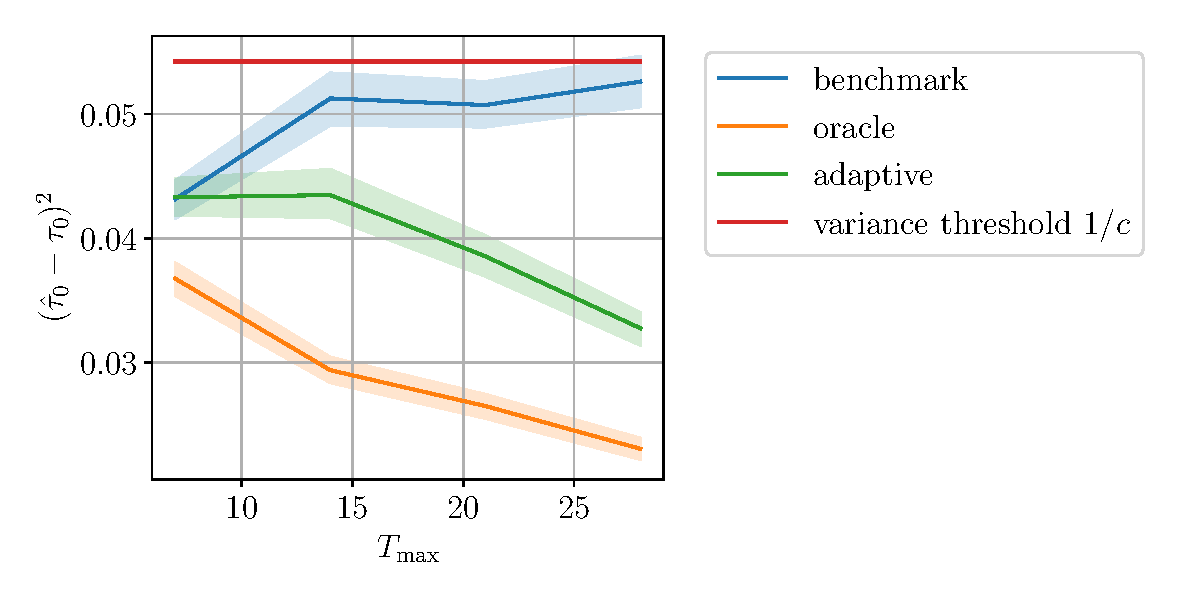
\includegraphics[width=1\linewidth]{plots/empirical/flu/adaptive/flu_adaptive_comparison-20.pdf}
		\caption{large threshold $c = 0.02 \cdot N/\tau_0^2$}
	\end{subfigure}
	\smallskip
	\caption{\textbf{Comparison of various designs in adaptive experiments with alternative thresholds} This figure shows the mean and 95\% confidence band of $(\hat{\tau}_0 - \tau_0)^2$ for adaptive, benchmark, and oracle designs, based on 10,000 synthetic adaptive experiments. 
	}
	\label{fig:various-opt-design-supp}
\end{figure}







